%% Assignment
%% 中文报告、作业报告、实验报告、文献
%%%%%%%%%%%%%%%%%%%%%%%%%%%%%%%%%%%%%%%%%

%----------------------------------------------------------------------------------------
%	PACKAGES AND OTHER DOCUMENT CONFIGURATIONS
%----------------------------------------------------------------------------------------

\documentclass[UTF8]{ctexart}
%%%%%%%%%%%%%%%%%%%%%%%%%%%%%%%%%%%%%%%%%
% Lachaise Assignment
% Structure Specification File
% Version 1.0 (26/6/2018)
%
% This template originates from:
% http://www.LaTeXTemplates.com
%
% Authors:
% Marion Lachaise & François Févotte
% Vel (vel@LaTeXTemplates.com)
%
% License:
% CC BY-NC-SA 3.0 (http://creativecommons.org/licenses/by-nc-sa/3.0/)
% 
%%%%%%%%%%%%%%%%%%%%%%%%%%%%%%%%%%%%%%%%%

%----------------------------------------------------------------------------------------
%	PACKAGES AND OTHER DOCUMENT CONFIGURATIONS
%----------------------------------------------------------------------------------------

\usepackage{amsmath,amsfonts,stmaryrd,amssymb} % Math packages

\usepackage{enumerate} % Custom item numbers for enumerations

\usepackage[ruled]{algorithm2e} % Algorithms

\usepackage[framemethod=tikz]{mdframed} % Allows defining custom boxed/framed environments

\usepackage{listings} % File listings, with syntax highlighting
\lstset{
	basicstyle=\ttfamily, % Typeset listings in monospace font
}
\usepackage{indentfirst}
\usepackage{bm}  %给数学符号加粗
\usepackage[colorlinks,  %引入超链接
linkcolor=black,
anchorcolor=black,
citecolor=black,
urlcolor=black
]{hyperref}
%----------------------------------------------------------------------------------------
%	DOCUMENT MARGINS
%----------------------------------------------------------------------------------------
%使图片、表格的编号按照section重新开始
%\usepackage{amsmath}
%\numberwithin{figure}{section}
%\numberwithin{table}{section}
%使section的标题左对齐
\CTEXsetup[format={\Large\bfseries}]{section}
\usepackage{geometry} % Required for adjusting page dimensions and margins

\geometry{
	paper=a4paper, % Paper size, change to letterpaper for US letter size
	top=2.5cm, % Top margin
	bottom=3cm, % Bottom margin
	left=2.5cm, % Left margin
	right=2.5cm, % Right margin
	headheight=14pt, % Header height
	footskip=1.5cm, % Space from the bottom margin to the baseline of the footer
	headsep=1.2cm, % Space from the top margin to the baseline of the header
	%showframe, % Uncomment to show how the type block is set on the page
}

\usepackage{fancyhdr}  %%设置页眉页脚
\pagestyle{fancy}   %风格为fancy(便于自己定义)
\fancyhead[L]{}  %左页眉为空
\fancyfoot{}   %页脚为空
\fancyfoot[C]{\thepage}  %页脚中间为页数
\renewcommand{\headrulewidth}{0pt} %去掉页眉下的横线

% 表格中支持跨行
\usepackage{multirow}

% 跨页表格
\usepackage{longtable}

% 固定宽度的表格
\usepackage{tabularx}

\usepackage{booktabs}

% 表格中的反斜线
\usepackage{diagbox}

% 确定浮动对象的位置,可以使用 H,强制将浮动对象放到这里(可能效果很差)
\usepackage{float}

%\usepackage{natbib}

\graphicspath{{figures/}}

%----------------------------------------------------------------------------------------
%	FONTS
%----------------------------------------------------------------------------------------
\usepackage{setspace}

\usepackage[utf8]{inputenc} % Required for inputting international characters
\usepackage[T1]{fontenc} % Output font encoding for international characters

\usepackage{XCharter} % Use the XCharter fonts
\usepackage{color}   %改变字体颜色
\usepackage{url}   %引用网址
\usepackage{bm}  %给数学符号加粗
\usepackage{subfigure} %have figures within figures
\usepackage{graphicx}
%\usepackage{wrapfig}  %插入图片
%----------------------------------------------------------------------------------------
%	COMMAND LINE ENVIRONMENT
%----------------------------------------------------------------------------------------

% Usage:
% \begin{commandline}
%	\begin{verbatim}
%		$ ls
%		
%		Applications	Desktop	...
%	\end{verbatim}
% \end{commandline}

\mdfdefinestyle{commandline}{
	leftmargin=10pt,
	rightmargin=10pt,
	innerleftmargin=15pt,
	middlelinecolor=black!50!white,
	middlelinewidth=2pt,
	frametitlerule=false,
	backgroundcolor=black!5!white,
	frametitle={Command Line},
	frametitlefont={\normalfont\sffamily\color{white}\hspace{-1em}},
	frametitlebackgroundcolor=black!50!white,
	nobreak,
}

% Define a custom environment for command-line snapshots
\newenvironment{commandline}{
	\medskip
	\begin{mdframed}[style=commandline]
}{
	\end{mdframed}
	\medskip
}

%----------------------------------------------------------------------------------------
%	FILE CONTENTS ENVIRONMENT
%----------------------------------------------------------------------------------------

% Usage:
% \begin{file}[optional filename, defaults to "File"]
%	File contents, for example, with a listings environment
% \end{file}

\mdfdefinestyle{file}{
	innertopmargin=1.6\baselineskip,
	innerbottommargin=0.8\baselineskip,
	topline=false, bottomline=false,
	leftline=false, rightline=false,
	leftmargin=2cm,
	rightmargin=2cm,
	singleextra={%
		\draw[fill=black!10!white](P)++(0,-1.2em)rectangle(P-|O);
		\node[anchor=north west]
		at(P-|O){\ttfamily\mdfilename};
		%
		\def\l{3em}
		\draw(O-|P)++(-\l,0)--++(\l,\l)--(P)--(P-|O)--(O)--cycle;
		\draw(O-|P)++(-\l,0)--++(0,\l)--++(\l,0);
	},
	nobreak,
}

% Define a custom environment for file contents
\newenvironment{file}[1][File]{ % Set the default filename to "File"
	\medskip
	\newcommand{\mdfilename}{#1}
	\begin{mdframed}[style=file]
}{
	\end{mdframed}
	\medskip
}

%----------------------------------------------------------------------------------------
%	NUMBERED QUESTIONS ENVIRONMENT
%----------------------------------------------------------------------------------------

% Usage:
% \begin{question}[optional title]
%	Question contents
% \end{question}

\mdfdefinestyle{question}{
	innertopmargin=1.2\baselineskip,
	innerbottommargin=0.8\baselineskip,
	roundcorner=5pt,
	nobreak,
	singleextra={%
		\draw(P-|O)node[xshift=1em,anchor=west,fill=white,draw,rounded corners=5pt]{%
		Question \theQuestion\questionTitle};
	},
}

\newcounter{Question} % Stores the current question number that gets iterated with each new question

% Define a custom environment for numbered questions
\newenvironment{question}[1][\unskip]{
	\bigskip
	\stepcounter{Question}
	\newcommand{\questionTitle}{~#1}
	\begin{mdframed}[style=question]
}{
	\end{mdframed}
	\medskip
}

%----------------------------------------------------------------------------------------
%	WARNING TEXT ENVIRONMENT
%----------------------------------------------------------------------------------------

% Usage:
% \begin{warn}[optional title, defaults to "Warning:"]
%	Contents
% \end{warn}

\mdfdefinestyle{warning}{
	topline=false, bottomline=false,
	leftline=false, rightline=false,
	nobreak,
	singleextra={%
		\draw(P-|O)++(-0.5em,0)node(tmp1){};
		\draw(P-|O)++(0.5em,0)node(tmp2){};
		\fill[black,rotate around={45:(P-|O)}](tmp1)rectangle(tmp2);
		\node at(P-|O){\color{white}\scriptsize\bf !};
		\draw[very thick](P-|O)++(0,-1em)--(O);%--(O-|P);
	}
}

% Define a custom environment for warning text
\newenvironment{warn}[1][Warning:]{ % Set the default warning to "Warning:"
	\medskip
	\begin{mdframed}[style=warning]
		\noindent{\textbf{#1}}
}{
	\end{mdframed}
}

%----------------------------------------------------------------------------------------
%	INFORMATION ENVIRONMENT
%----------------------------------------------------------------------------------------

% Usage:
% \begin{info}[optional title, defaults to "Info:"]
% 	contents
% 	\end{info}

\mdfdefinestyle{info}{%
	topline=false, bottomline=false,
	leftline=false, rightline=false,
	nobreak,
	singleextra={%
		\fill[black](P-|O)circle[radius=0.4em];
		\node at(P-|O){\color{white}\scriptsize\bf i};
		\draw[very thick](P-|O)++(0,-0.8em)--(O);%--(O-|P);
	}
}

% Define a custom environment for information
\newenvironment{info}[1][Info:]{ % Set the default title to "Info:"
	\medskip
	\begin{mdframed}[style=info]
		\noindent{\textbf{#1}}
}{
	\end{mdframed}
}
 % Include the file specifying the document structure and custom commands

%----------------------------------------------------------------------------------------
%	ASSIGNMENT INFORMATION
%----------------------------------------------------------------------------------------

\title{降雨量预测} % Title of the assignment

\author{孟诗涵$\;\;$2019211246\\ \texttt{mengsh19@mails.tsinghua.edu.cn}} % Author name and email address

\date{} % University, school and/or department name(s) and a date

%----------------------------------------------------------------------------------------

\begin{document}\normalsize

\maketitle % Print the title
\setlength{\baselineskip}{18pt}
%----------------------------------------------------------------------------------------

\section{简介}
\subsection{降水量预测任务及主流的解决方法}
降水量任务多年来受到广泛关注,属于时空序列类预测问题。各领域研究人员提出了很多不同的模型,著名的有**,**和**。

\subsection{机器学习方法在降水量预测中的应用,调研5篇文档}

\subsection{本文主要贡献}

\section{任务定义}
本文将降水量预测问题定义为分类问题,根据**按照降水量的数值分成无雨,小雨,中雨和大到暴雨四类。同时,本文将问题定义为短时预测问题,基于前六小时的特征数据预测下一小时的降水量,对5个邻近气象站分别单独建模。

\subsection{符号公式定义}

\section{数据整理}

\subsection{数据来源,内容}

数据集来自巴西国家气象研究所(INMET)【\cite{kaggle网站}】,它涵盖了来自东南地区(巴西)的122个气象站从2000年到2016年的每小时天气观测数据(并非所有气象站都是从2000年开始观测的)。东南部包括里约热内卢,圣保罗,米纳斯吉拉斯州和圣埃斯皮里图州等。数据是由维萨拉自动气象站AWS310自动捕捉,所以可能发生设备故障导致数据错误或缺失的情况。整个数据集规模为9779168条信息,31个特征。 其中有时间地点,气象站编号等信息,还有17个气象数据分别为temp-瞬时空气温度(摄氏度)、tmax-最高气温(摄氏度)、tmin-最低气温(摄氏度)、hmdy-空气相对湿度(%)。hmax-最大相对空气湿度(%)、hmin-最低相对空气湿度(%)、dewp-即时露点(摄氏度)、dmax-最大露点(摄氏度)、dmin-最低露点温度(摄氏度)、stp-瞬时大气压(百帕)、smax-最大大气压(百帕)、smin-最低大气压(百帕)、wdsp-瞬时风速(米/秒)、wdct-风向(半径度)、gust-阵风强度(米/秒)、gbrd-太阳辐射、prcp-降水量(毫米)。

首先观察气象数据的分布,最大值最小值应与实际值有类似的分布,具体见图\ref{fig:1}。其中所有特征均有较多的零值,需要逐一分析,并进行对应的清洗。需要预测的prcp-降水量绝大部分都是0值,非常稀疏,给预测带来了很大的困难。stp-气压、temp-温度、dewp-露点温度基本为正态分布,数值保持在一个范围之内。考虑到夜晚没有太阳照射,gbrd-太阳辐射绝大部分值为0,低辐射值分布略比高辐射值大,中辐射值分布比较均匀。hmdy-空气湿度数值从100\%降低,分布越来越少。风速是一个均值偏向0的正态分布。

\begin{figure}[htbp]
\label{fig:1}
\centering

\subfigure[prcp-降水量]{
\begin{minipage}[t]{0.33\linewidth}
\centering
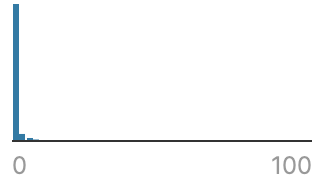
\includegraphics[width=0.8\textwidth]{1-1.png}
%\caption{fig1}
\end{minipage}%
}%
\subfigure[stp-气压]{
\begin{minipage}[t]{0.33\linewidth}
\centering
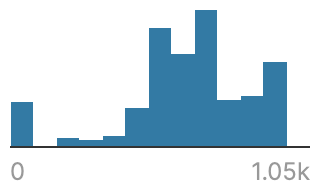
\includegraphics[width=0.8\textwidth]{1-2.png}
%\caption{fig2}
\end{minipage}%
}%        
\subfigure[gbrd-太阳辐射]{
\begin{minipage}[t]{0.33\linewidth}
\centering
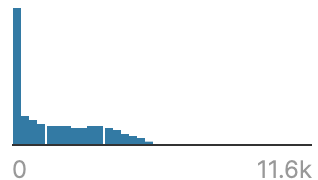
\includegraphics[width=0.8\textwidth]{1-3.png}
%\caption{fig2}
\end{minipage}
}%
\quad  
\subfigure[temp-空气温度]{
\begin{minipage}[t]{0.33\linewidth}
\centering
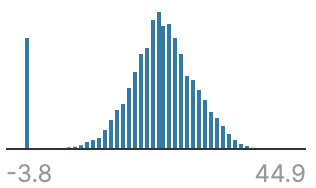
\includegraphics[width=0.8\textwidth]{1-4.png}
%\caption{fig2}
\end{minipage}
}%
\subfigure[dewp-露点温度]{
\begin{minipage}[t]{0.33\linewidth}
\centering
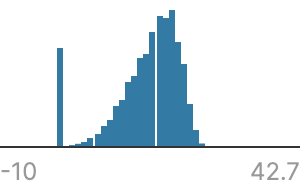
\includegraphics[width=0.8\textwidth]{1-5.png}
%\caption{fig2}
\end{minipage}
}%
\subfigure[hmdy-空气相对湿度]{
\begin{minipage}[t]{0.33\linewidth}
\centering
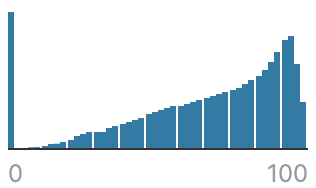
\includegraphics[width=0.8\textwidth]{1-6.png}
%\caption{fig2}
\end{minipage}
}%
\quad
\subfigure[wdsp-瞬时风速]{
\begin{minipage}[t]{0.33\linewidth}
\centering
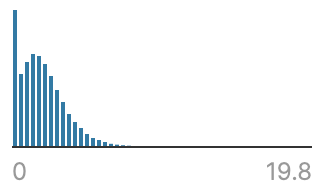
\includegraphics[width=0.8\textwidth]{1-7.png}
%\caption{fig2}
\end{minipage}
}%
\subfigure[wdct-风向]{
\begin{minipage}[t]{0.33\linewidth}
\centering
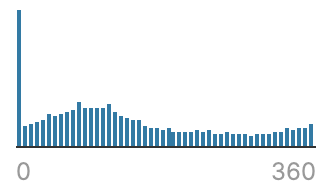
\includegraphics[width=0.8\textwidth]{1-8.png}
%\caption{fig2}
\end{minipage}
}%
\subfigure[gust-阵风]{
\begin{minipage}[t]{0.33\linewidth}
\centering
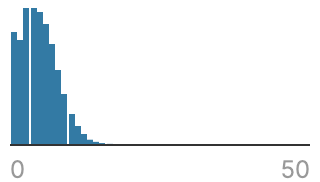
\includegraphics[width=0.8\textwidth]{1-9.png}
%\caption{fig2}
\end{minipage}
}%

\centering
\caption{各气象特征数据分布直方图}
\end{figure}

\subsection{数据清洗及处理}

对不同的参数有不同的处理。其中降水量和太阳能将nan值用0替代,作为可用数据条。Stp,smax,smin表示气压值,temp,tmax,tmin, dewp, dmax, dmin表示温度,hmdy, hmax, hmin表示湿度,wdsp,wdct,gust表示风速有关的数据。上述特征值均为连续实数,将nan值用0替代后做线性插值,但是线性插值对长时间一整段的数据缺失无用,所以直接将一整段数据丢失的样本丢弃。

有一个气象站的经纬度及海拔信息缺失,谷歌出正确的信息补全。另外有两个气象站经纬度信息错误,改正。

考虑到计算机算力问题,在122个气象站中根据数据量排序选择编号为371-375的五个气象站,它们均在RJ省,经纬度上看为邻近的城市,海拔均在100米以下,靠近海边,受热带气候影响,降雨量较多,一定程度上缓解数据稀疏问题,有利于模型分类。


\section{特征提取}

\subsection{数据归一化处理}
采用sklearn包中standardScaler对数据统一进行归一化处理,变为标准正态分布。即默认训练集验证集测试集同分布。本文采用的某些模型对归一化不敏感,有些则很敏感,具体分析见章节?。

\subsection{最终使用的特征维度和每一维的含义}
气象数据中大气压、温度、湿度在一个小时内基本稳定,所以将最大值最小值丢弃,只采用stp、temp、dewp、hmdy、wdsp、wdct、gust等进行建模。保留时间特征,因为时间序列中时间是非常重要的特征,反应了待预测数据量的变化信息。另外考虑到五个气象站的不同,保留地理位置等信息,最终单个气象站模型使用的特征共13维,具体见表\ref{tab:特征}。在章节?会讨论全部特征和进行选择后的部分特征对结果造成的影响。

\begin{table}[htb]
  \centering
  \begin{minipage}[t]{0.4\linewidth}
  \caption{最终使用的特征}
  \label{tab:特征}
    \begin{tabular}{cc}
      \toprule[1.5pt]
      特征名称& {特征含义} \\
      \midrule[1pt]
      {yr} & 年 \\
      {mo} & 月  \\
      {da} & 日 \\
      {hr} & 小时  \\
      {stp} & 气压 \\
      {gbrd} & 太阳辐射 \\
      {temp} & 空气温度 \\
      {dewp} & 露点温度 \\
      {hmdy} & 空气相对湿度 \\
      {wdsp} & 瞬时风速 \\
      {wdct} & 风向 \\
      {gust} & 阵风强度 \\
      {prcp} & 过去一小时降水量 \\
      \bottomrule[1.5pt]
    \end{tabular}
  \end{minipage}
\end{table}

\subsection{特征相关性}
在整个数据集上观察各个特征维度与预测值降水量的相关性,得到结果如图\ref{fig:corr}所示。由图可得到以下结论:
\begin{itemize}
	\item 最大值最小值相关性基本与实际值相等,说明之前的特征选择操作是合理的;
	\item 湿度hmdy,阵风gust等与降水量prcp正相关;太阳辐射gbrd,温度temp,气压stp与降水量prcp负相关,即风大气压低更有可能下雨,基本符合常识;
	\item 时间,经纬度和气象站信息相关性相对不明显。
\end{itemize}


\begin{figure}[h] % use float package if you want it here
  \centering
  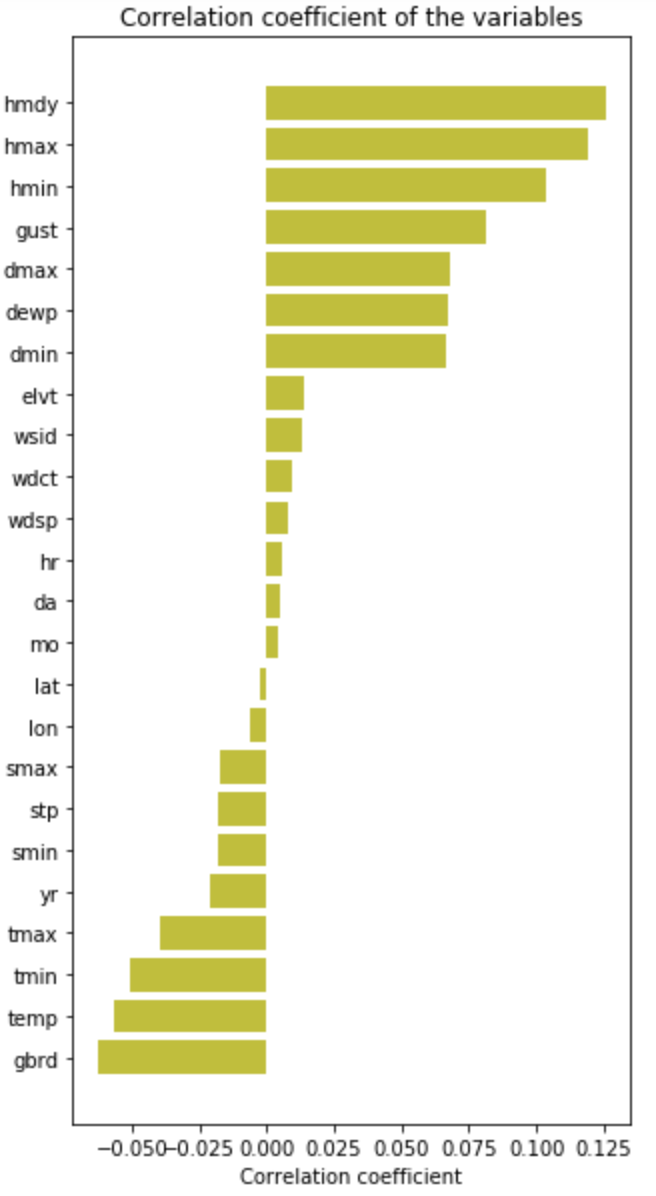
\includegraphics[width = 0.4\textwidth]{corr.png}
  \caption{特征相关性}
  \label{fig:corr}
\end{figure}

因为降水量为时间序列,为了观察时序上的相关性,以温度temp和湿度hmdy为例,得到相关性热度图如图\ref{fig:timelag}所示。可以得到如下结论:
\begin{itemize}
	\item 湿度hmdy和温度temp均有明显的时间正相关性,时间越近相关性越大,接近1;
	\item 湿度hmdy和温度temp有明显的负相关性。
\end{itemize}

\begin{figure}[h] % use float package if you want it here
  \centering
  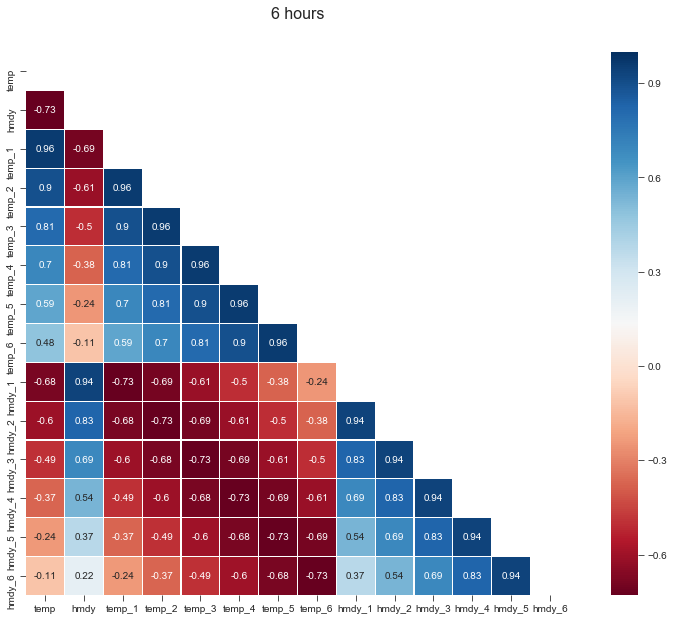
\includegraphics[width = 0.8\textwidth]{time-lag.png}
  \caption{6小时内温度和湿度相关性热度图}
  \label{fig:timelag}
\end{figure}



\section{模型设计}

\subsection{线性模型}

\subsubsection{逻辑回归分类器Logistic Regression Classifier}

逻辑回归假设数据服从伯努利分布,通过极大化似然函数方法,运用梯度下降来求解参数,来达到将数据二分目的。多分类器可由二分类器推广得到。本质上是一个线性模型,可利用特征核函数将低维特征映射到高维,类似支持向量机(SVM)。

【解决欠拟合和过拟合的问题,欠拟合可以增加特征维度,过拟合可以减小特征维度,正则化,逐渐减小梯度下降学习率等方法来解决。】

逻辑回归分类器具有如下优点:
\begin{enumerate}[(1)]
	\item 直接对分类的可能性建模,无需事先假设数据分布,避免了假设分布不准确带来的问题。同时对率函数是任意阶可导凸函数,有很好得数学性质,很多数值优化算法可直接用于求取最优解;
	\item 不仅预测出类别,还可得到近似概率预测,因此可用作排序模型;
	\item 算法简单,容易使用和解释,计算代价低,可应用于分布式数据和在线算法实现,用较小资源处理较大数据;
	\item 算法稳定性高,对数据中小噪声鲁棒性很好,并且不会受到轻微多重共线性影响。
\end{enumerate}

缺点:
\begin{enumerate}[(1)]
	\item 容易欠拟合,分类精度不高;
	\item 数据特征有缺失或特征空间很大时效果不好。
\end{enumerate}


\subsubsection{SVM}
支持向量机(support vector machine,SVM)是一种二分类模型,可推广到多分类器。其基本模型定义是特征空间上的间隔最大的线性分类器(当采用线性核时),即支持向量机的学习策略是间隔最大化,最终可转化为一个凸二次规划问题的求解。对于线性不可分问题,可利用核函数将低维特征映射到高维,再进行划分。

支持向量机算法具有如下优点:
\begin{enumerate}[(1)]
	\item SVM算法简单,易于理解,核心为最大化分类边界,得到支持向量;
	\item SVM 的最终决策函数只由少数的支持向量所确定,计算的复杂性取决于支持向量的数目,而不是样本空间的维数,这在某种意义上避免了“维数灾难”;
	\item 少数支持向量使算法具有较好的稳定性,比如增删非支持向量样本对模型没有影响。
\end{enumerate}

缺点:
\begin{enumerate}[(1)]
	\item 通过二次规划来求解计算复杂度高,大样本时所需时间长;
	\item 非线性问题的核函数难以选择;
	\item 对缺失数据敏感。
\end{enumerate}


\subsubsection{KNN}
KNN是近邻法的一种,核心思想为一个样本的分类结果与它周围的邻居类别有关,通过投票法等方法确定该样本的类别。

近邻法具有如下优点:
\begin{enumerate}[(1)]
	\item 算法简单,易于理解,易于实现,无需估计参数,无需训练;
	\item 适合于多分类问题(multi-modal,对象具有多个类别标签)。
\end{enumerate}

缺点:
\begin{enumerate}[(1)]
	\item 需要存储所有样本的距离矩阵,计算量大,内存开销大;
	\item 样本不平衡时,对稀有类别的预测准确率低;
	\item 相比于决策树模型,可解释性不强。
\end{enumerate}


\subsection{树模型}

\subsubsection{Decision Tree}
决策树是基于规则进行决策和判别的树模型,目的是构造一棵泛化能力强的树。它采用自顶向下的递归方式来生长。随着树的生长,完成对训练样本集的不断细分,最终都被细分到了每个叶子结点上。


决策树具有如下优点:
\begin{enumerate}[(1)]
	\item 对噪声数据具有很好的鲁棒性,且对缺失值不敏感,能处理连续离散等多种属性的数据;
	\item 效率高,运行时间短,一旦构建完决策树模型,可以多次使用;
	\item 学习得到的决策树可以表示为多条if-then形式的决策规则,因此具有很强的可读性和可解释性。
\end{enumerate}

缺点:
\begin{enumerate}[(1)]
	\item 容易导致过拟合,需要剪枝等操作,或者采用随机森林模型;
	\item 容易忽略数据集中属性的相互关联,特别是在本文的时间序列模型中;
	\item 样本不均衡时,不同的判定准则会有不同的属性偏向:比如信息增益准则对数目较多的属性有所偏好(典型代表ID3算法),而增益率准则(CART)则对数目较少的属性有所偏好。
\end{enumerate}


\subsubsection{Random Forest}
随机森林是一个用随机方式建立的,包含多个决策树的分类器,也属于集成学习中的bagging算法的一种。随机性主要体现在两个方面:一是重采样,训练每棵树时,从全部训练样本(样本数为N)中选取一个可能有重复的大小同样为N的数据集进行训练(即bootstrap取样);二是随机选取特征,在每个节点,随机选取所有特征的一个子集,用来计算最优分类特征。

随机森林在决策树优缺点的基础上,具有不易过拟合,可以降低方差等优点,同时对于样本不均衡的问题,它可以平衡误差。


\subsubsection{GBDT}
GBDT是梯度下降与决策树模型的结合,是一种boosting方法,每一次建立模型,是在之前建立模型损失函数的梯度下降方向。

GBDT在决策树的基础上具有如下优点:
\begin{enumerate}[(1)]
	\item 具有boosting思想,每一步的残差计算其实变相地增大了分错实例(instance)的权重,而已经分对的实例(instance)则都趋向于0。这样后面的树就能越来越专注那些前面被分错的实例(instance);
	\item 表达能力强,无须对特征进行复杂的变换和选择,且能够自动对特征重要性排序。
\end{enumerate}

缺点:
\begin{enumerate}[(1)]
	\item Boost是一个串行过程,不好并行化,计算复杂度高;
	\item 不太适合高维稀疏特征,如果feature个数太多,每一棵回归树都要耗费大量时间,甚至不如SVM。
	
\end{enumerate}


\subsubsection{Xgboost}


\subsection{神经网络模型}

\subsubsection{MLP}
MLP多层感知机是一种前馈神经网络,基于反向梯度传播学习。

MLP具有如下优点:
\begin{enumerate}[(1)]
	\item 高度的并行处理,算法效率高
	\item 有很强的自适应,自学习的能力。
\end{enumerate}

缺点:
\begin{enumerate}[(1)]
	\item 具有神经网络模型的统一缺点,可解释性较差;
	\item 网络隐含层的参数选取比较困难,容易陷入局部极值。
	
\end{enumerate}


\subsubsection{LSTM}


\subsection{集成方法}
三个臭皮匠顶个诸葛亮。在集成方法中,我们训练多个弱学习器模型以解决相同的问题,并将它们结合起来从而获得更好的结果。当弱学习期被正确组合时,可以得到更精确更鲁棒的模型。在bagging和boosting等方法中,我们使用多个同一种基学习器,加入随机因子,用不同的方法训练;也可以使用不同种类的基学习器。
\subsubsection{平均方法average}
投票分类器是将不同的基学习器组合,并使用多数表决或平均预测概率来预测类标签。这样的分类器可用于一组性能良好的模型,以平衡其各自的弱点。
本文采用单独模型中的LR、SVM、KNN、RF、MLP生成组合模型,分别采用多数表决(hard)和平均预测概率(soft)两种方法实现。

用sklearn包中votingclassifier实现。

\subsubsection{增强方法boosting}



\section{实验设计及结果}

\subsection{数据集划分}
X-train(n\_samples, 78)的说明,gridsearchcv中因为cv=5,所以只分训练集和测试集即可,交叉验证会自动从训练集中分出验证集。

\subsection{评价指标的定义}
precision, recall, fscore三个指标,含义?。用sklearn包中的classification\_report直接得到。

\subsection{每种模型单独的最好结果对比} 
从表\ref{tab:单独模型}所示,共九种模型的四个指标。每一个单元格中从左到右分别为371-375五个气象站的结果,可以看到在同一个气象站数据下,不同模型的四个指标都有类似的数值,即不同气象站的指标具有不同的均值和方差,说明分类结果与数据集本身分布相关。标黑的数值表示在同一个气象站数据下,最优的模型表现,综合来看GBDT的性能最优。整体来看,各个模型的性能指标都类似,只有小幅的偏差,可能说明分类器的性能均已达到比较优的情况。另外,在accuracy,precision,recall,fscore里,precision和fscore数值上相对稍低,recall相对稍高。
\begin{table}[htb]
  \centering
  \begin{minipage}[t]{\linewidth}
  \centering
  \caption{单独模型的最好结果对比}
  \label{tab:单独模型}
    \begin{tabular}{ccccc}
      \toprule[1pt]
      模型 & accuracy & precision & recall & f1-score \\
      \midrule[0.5pt]
      LR & .93|.93 |.89|.96|.95 & .90|.90|.83|.93|.93& .93|.93|.89|.96|.95& .91|.91|.84|.94|.93 \\
      SVM & .93|.93|.89|.96|.95& .91|.90|.84|.93|.92& .93|.93|.89|.96|.95 & .91|.91|.85|.94|.92 \\
      KNN & .93|.92|.88|.96|.95 & .90| .89|.83|.93|.91& .93|.93|.88|.96|.94& .91|.90|.85|.94|.92 \\
      DT & .93|.93|.90|.96|.95 &.91|\textbf{.92}|.87|\textbf{.95}|.93& .93|.93|.90|.96|.95& .92|.92|.88|.95|.94 \\
      RF & .93|.93|.90|.96|.94 & .91|.91|.87|.94|.93 & .93|.93|.90|.95|.94 & .92|.92|.88|.95 |.94\\
      GBDT & .94|.93|.90|.96|.95 &\textbf{.92}|\textbf{.92}|\textbf{.88}|\textbf{.95}|\textbf{.94}& \textbf{.94}|.93|.90 |.96|.95 & \textbf{.93}|.92|\textbf{.89}|.95|.94 \\
      MLP & .94|.93|.90|.96|.95 &\textbf{.92}|.91|.87|\textbf{.95}|\textbf{.94}& \textbf{.94}|.93|.90|.96|.95& \textbf{.93}|.92|.88|.95|.94 \\
      \bottomrule[1pt]
    \end{tabular}
  \end{minipage}
\end{table}

\subsection{ensemble后的最好结果对比}
以375气象站为例,emsemble后结果见表\ref{tab:ensemble模型}所示。ensemble后模型性能与最优的单个模型齐平,没有明显的提升。可能是单个模型已经有很好的性能了。
\begin{table}[htb]
  \centering
  \begin{minipage}[t]{\linewidth}
    \centering
  \caption{不同ensemble模型的最好结果对比}
  \label{tab:ensemble模型}
    \begin{tabular}{ccccc}
      \toprule[1pt]
      模型 & accuracy & precision & recall & f1-score \\
      \midrule[0.5pt]
      hard-voting & .95& .93& .95& .94\\
      soft-voting &  .95& .92&.95 &.93 \\
      \bottomrule[1pt]
    \end{tabular}
  \end{minipage}
\end{table}


\subsection{不同超参数对模型的影响}
上述模型均为机器学习经典模型,且在上课和课后作业中讨论过不同超参数的影响,不再赘述。此节讨论class\_weight这一参数对模型的影响。

由上述章节?可知降水量数据具有稀疏性,导致分类后样本极度不均衡,由此训练出的分类器可能有较高的准确性但是性能较差。为了解决这一问题,可以采用以下几种措施:

\begin{itemize}
	\item 扩大数据集,对稀有样本重采样,对多数样本进行欠采样;
	\item 采用更合理的评价指标,比如本文中采用的precision、recall和f1-score;
	\item 尝试不同的分类算法,比如决策树模型等常在类别不均衡的问题上有较好的表现;
	\item 对问题重新定义,可将小类样本作为异常点,因此该问题即转化为异常点检测(anomaly detection)与变化趋势检测问题(change detection);
	\item 采用代价敏感学习方法,给少数类样本分配较高的误分类代价,而给多数类样本分配较小的误分类代价,通过这种方式在训练中人为提高了少数类别样本的重要性,以此减轻分类器对多数类的偏好。
	\item 采用集成方法。

\end{itemize}

本文对LR,SVM,DT三种算法进行样本均衡,设置class\_weight参数为‘balanced’,根据样本数量确定权重,以372气象站为例,得到结果如下表\ref{tab:class}所示。
可以看到LR对样本均衡问题不敏感,而SVM和DT则有较大变化。SVM增加了样本权重后,accuracy大幅降低,precision稍有上升,recall和fscore均下降。DT同样accuracy大幅降低,precision,recall和fscore均下降。这是由模型特点决定的,LR不会受到小噪声的影响;SVM对于不同代价函数敏感,可能会导致不同的边界和支持向量;单棵DT由于样本不均衡会产生一定的偏向,这一问题能够在森林中解决。
另外,对于数据集的进一步清洗,包括删除缺失属性的数据条等操作,能够提高balanced后的模型性能,这可能是因为清洗的绝大部分是0类,一定程度上改善了样本不均衡的问题。

\begin{table}[htb]
  \centering
  \begin{minipage}[t]{0.9\linewidth}
  \centering
  \caption{class\_weight超参数结果对比}
  \label{tab:class}
    \begin{tabular}{ccccc}
      \toprule[1pt]
      模型 & accuracy & precision & recall & f1-score \\
      \midrule[0.5pt]
      LR & .93 & .90 & .93 & .91\\
      LR(balanced) &  .91 & .92 &.91 &.92 \\
      SVM &.93 &.9 &.93 & .91   \\
      SVM(balanced) & .79 & .92& .79& .84 \\
      DT & .93 & .92 & .93 & .92\\
      DT(balanced) & .83 &.91 &.83 &.87 \\
      \bottomrule[1pt]
    \end{tabular}
  \end{minipage}
\end{table}



\section{实验结果分析}

【讨论数据和模型中每一部分的贡献:正则化standardScale?one-hot?】


\subsection{特征重要性分析}
利用随机森林分类结果,可以得到特征重要性排序,前十个特征由下表\ref
{tab:rf特征重要性}所示,其中特征前的数字表示前$6-n$小时的值。
\begin{table}[htb]
  \centering
  \begin{minipage}[t]{0.9\linewidth}
  \centering
  \caption{特征重要性分析}
  \label{tab:rf特征重要性}
    \begin{tabular}{ccc}
      \toprule[1pt]
       & 特征 & 重要性  \\
      \midrule[0.5pt]
      1 & 5prcp & 0.217  \\
      2 & 4prcp & 0.156 \\
      3 & 3prcp & 0.143  \\
      4 & 2prcp & 0.097\\
	  5 & 5hmdy & 0.016  \\
	  6 & 5gbrd & 0.016  \\
      7 & 4hmdy & 0.016 \\
      8 & 5temp & 0.015\\
	  9 & 5wdct & 0.014  \\
      10 & 4gbrd & 0.012 \\
      \bottomrule[1pt]
    \end{tabular}
  \end{minipage}
\end{table}


上述结果均由用章节?的特征子集得到,考虑把所有数值特征不经过特征选择,直接输入模型中,可以观察到结果基本相似,甚至略有提升。

另外,不清洗缺失某些数据值的数据条,也会得到略有提升的模型性能。可能是因为缺失的特征对于分类的重要性不高,保留使得数据集样本规模更大,所以会有更好的性能。


【错误分析,】


【案例分析】

\subsection{回归问题}
采用LR,SVR等线性模型,用R2、RMSE、MAE等指标进行评价,只能得到R2接近0的性能,基本与随机猜测没有区别,所以选择重新定义问题为分类问题。


【模型和结果可视化分析?】

【参考文献】


\end{document}
